%%%%%%%%%%%%%%%%%%%%%%%%%%%%% Define Article %%%%%%%%%%%%%%%%%%%%%%%%%%%%%%%%%%
\documentclass[conference]{IEEEtran}
%%%%%%%%%%%%%%%%%%%%%%%%%%%%%%%%%%%%%%%%%%%%%%%%%%%%%%%%%%%%%%%%%%%%%%%%%%%%%%%

%%%%%%%%%%%%%%%%%%%%%%%%%%%%% Using Packages %%%%%%%%%%%%%%%%%%%%%%%%%%%%%%%%%%
\usepackage{graphicx}
\usepackage{amssymb}
\usepackage{amsmath}
\usepackage{amsthm}
\usepackage{booktabs}
\usepackage{pgfplots}
\usepackage{bm}
\usepackage[spanish]{babel}
\usepackage{caption}
\usepackage{multirow}
\usepackage{subcaption}
\usepackage{hyperref}
%%%%%%%%%%%%%%%%%%%%%%%%%%%%%%%%%%%%%%%%%%%%%%%%%%%%%%%%%%%%%%%%%%%%%%%%%%%%%%%

%%%%%%%%%%%%%%%%%%%%%%%%%%%%%%% Plotting Settings %%%%%%%%%%%%%%%%%%%%%%%%%%%%%
\pgfplotsset{width=8cm,compat=1.9}
%%%%%%%%%%%%%%%%%%%%%%%%%%%%%%%%%%%%%%%%%%%%%%%%%%%%%%%%%%%%%%%%%%%%%%%%%%%%%%%

%%%%%%%%%%%%%%%%%%%%%%%%%%%%%%% Title & Author %%%%%%%%%%%%%%%%%%%%%%%%%%%%%%%%
\title{Diseño, análisis y simulación de una instalación eléctrica de iluminación con conexiones serie y paralelo}

\author{
  \IEEEauthorblockN{Nombre Apellido, Otro Nombre Apellido}
  \IEEEauthorblockA{Escuela E3T, Universidad Industrial de Santander\\
  Correo: \{usuario1, usuario2\}@correo.uis.edu.co}
}
%%%%%%%%%%%%%%%%%%%%%%%%%%%%%%%%%%%%%%%%%%%%%%%%%%%%%%%%%%%%%%%%%%%%%%%%%%%%%%%

\begin{document}

\maketitle

%% ─── Resumen ───────────────────────────────────────────────────────────────
\begin{abstract}
Este artículo presenta el diseño, análisis y simulación de un sistema de iluminación para [nombre del espacio real, ej. “una oficina de 30 m²”] utilizando conexiones en serie y en paralelo. Se realizó un levantamiento de campo (medidas, tipo de lámparas, ubicación de interruptores, croquis), se elaboraron planos arquitectónico y eléctrico, y se calcularon variables eléctricas (corriente, voltaje, resistencia equivalente, potencia, consumo). Los circuitos se simularon en software [nombre del software, ej. “LTspice”] para validar su comportamiento. Los resultados muestran que la conexión en paralelo garantiza independencia de lámparas y estabilidad de tensión, mientras que la serie presenta caída de tensión y dependencia total. Se concluye que la instalación real debe emplear topología paralela.
\end{abstract}


\begin{IEEEkeywords}
  Tectonic, IEEEtran, LaTeX, pgfplots, BibTeX.
\end{IEEEkeywords}

%% ─── Contenido ──────────────────────────────────────────────────────────────

\section{Introducción}
El alumbrado eléctrico representa una fracción significativa del consumo energético en edificaciones. El diseño correcto de circuitos de iluminación requiere aplicar leyes fundamentales (Ohm, Kirchhoff) y elegir la topología adecuada. Este proyecto integra los conceptos de Circuitos Eléctricos I mediante el estudio de caso de [nombre del espacio], comparando conexiones serie y paralelo. El informe sigue el formato IEEE y normas APA.

\section{Objetivos}
\subsection{Objetivo general}
Diseñar, analizar y simular una instalación eléctrica de iluminación para [nombre del espacio], aplicando conexiones en serie y en paralelo.

\subsection{Objetivos específicos}
\begin{itemize}
    \item Realizar el levantamiento de información del lugar (medidas, luminarias existentes, interruptores, cableado).
    \item Elaborar el plano arquitectónico y el diseño eléctrico (serie y paralelo) con simbología normalizada.
    \item Calcular corriente, voltaje, resistencia equivalente, potencia de cada lámpara y consumo total.
    \item Simular el comportamiento de ambos circuitos en un software especializado.
    \item Comparar ventajas y desventajas técnicas de cada topología.
\end{itemize}

\section{Justificación}
La selección incorrecta de la conexión de luminarias puede causar bajo rendimiento luminoso, caídas de tensión o fallos en cascada. Este proyecto permite aplicar directamente las leyes de circuitos eléctricos a un caso real, desarrollando competencias de diseño, cálculo y simulación. Además, los resultados servirán para recomendar la mejor práctica en instalaciones de iluminación.

\section{Marco teórico}
\subsection{Leyes fundamentales}
La Ley de Ohm establece \( V = I \cdot R \). Las leyes de Kirchhoff: (1) Ley de nodos: \(\sum I_{\text{ent}} = \sum I_{\text{sal}}\); (2) Ley de mallas: \(\sum V = 0\). La potencia eléctrica se calcula como \( P = V \cdot I = I^2 R = V^2 / R \).

\subsection{Conexiones serie y paralelo}
En serie, la corriente es la misma en todos los elementos, el voltaje se divide y la resistencia equivalente es \( R_{eq} = R_1 + R_2 + \dots + R_n \). Una falla en una lámpara abre el circuito. En paralelo, el voltaje es común, la corriente se divide y \( 1/R_{eq} = 1/R_1 + 1/R_2 + \dots + 1/R_n \). Las lámparas operan independientemente.

\subsection{Simulación de circuitos}
La simulación permite validar el diseño antes de la implementación física. Software como LTspice, Multisim o Proteus resuelven las ecuaciones de red y muestran tensiones, corrientes y potencias.

\section{Metodología}
Se siguieron cuatro fases:
\begin{enumerate}
    \item \textbf{Investigación y levantamiento de información}: visita al lugar, medición de dimensiones, registro fotográfico, identificación de luminarias, interruptores y cableado, elaboración de croquis preliminar.
    \item \textbf{Diseño arquitectónico y eléctrico}: creación del plano arquitectónico (con medidas reales) y de dos diagramas eléctricos (serie y paralelo) con simbología IEC/ANSI. Cálculo de todas las variables eléctricas.
    \item \textbf{Simulación}: implementación de ambos circuitos en [software], verificación de encendido/apagado y medición de voltajes/corrientes.
    \item \textbf{Análisis e informe}: comparación de resultados, redacción del artículo en formato IEEE, inclusión de planos, tablas y capturas.
\end{enumerate}

\section{Desarrollo del diseño eléctrico}
\subsection{Descripción del lugar}
El espacio seleccionado es [nombre del lugar, ej. “una sala de reuniones”] con dimensiones: largo [X] m, ancho [Y] m, altura [Z] m. El sistema de iluminación existente consta de [número] lámparas [tipo, ej. “LED de 10 W”] ubicadas en [ubicación]. Los interruptores son [tipo, ej. “unipolares”] y el cableado visible es [calibre, material]. En la Figura \ref{fig:croquis} se muestra el croquis preliminar.

\begin{figure}[h]
\centering
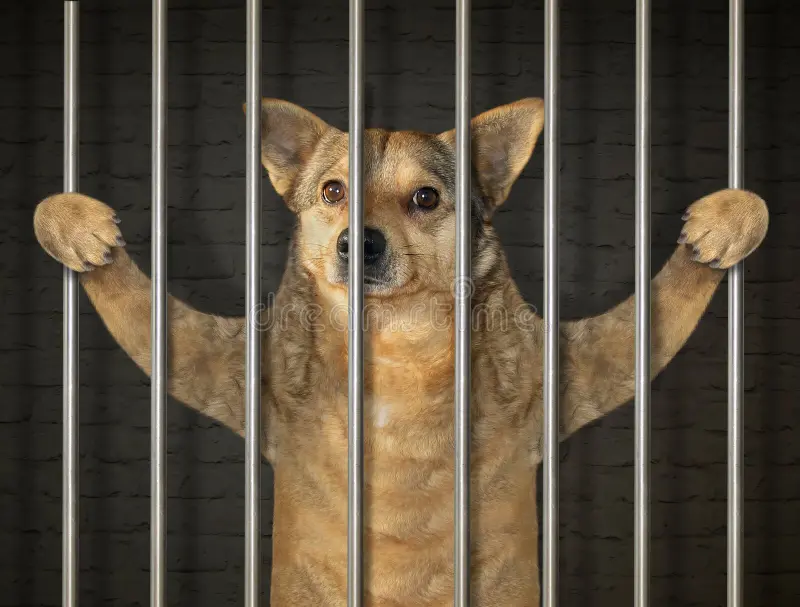
\includegraphics[width=0.6\linewidth]{croquis.png}
\caption{Croquis preliminar del espacio.}
\label{fig:croquis}
\end{figure}

La Tabla \ref{tab:medidas} resume las áreas.

\begin{table}[h]
\centering
\caption{Medidas y áreas del lugar.}
\label{tab:medidas}
\begin{tabular}{|l|c|}
\hline
\textbf{Parámetro} & \textbf{Valor} \\
\hline
Largo & [X] m \\
Ancho & [Y] m \\
Altura & [Z] m \\
Área total & [X*Y] m² \\
\hline
\end{tabular}
\end{table}

\subsection{Plano arquitectónico y eléctrico}
El plano arquitectónico (Figura \ref{fig:plano_arq}) se elaboró con AutoCAD (o herramienta similar) respetando las medidas reales. El diseño eléctrico incluye:
\begin{itemize}
    \item \textbf{Conexión serie}: tres lámparas de 60 W / 120 V conectadas en serie a una fuente de 120 V.
    \item \textbf{Conexión paralelo}: las mismas tres lámparas conectadas en paralelo a la misma fuente.
\end{itemize}
La simbología utilizada (interruptor, lámpara, conductor, fuente) se muestra en el plano eléctrico (Figura \ref{fig:plano_elec}).

\begin{figure}[h]
\centering
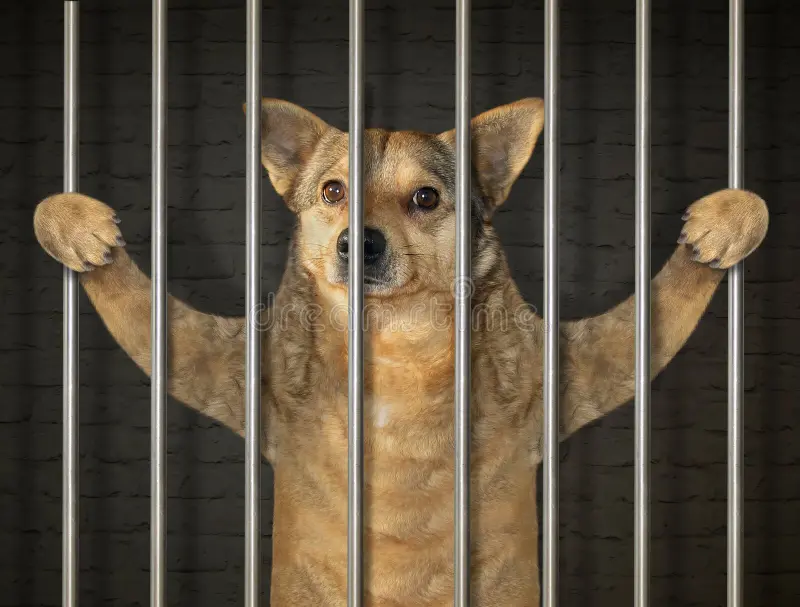
\includegraphics[width=0.8\linewidth]{plano_arquitectonico.png}
\caption{Plano arquitectónico del espacio.}
\label{fig:plano_arq}
\end{figure}

\begin{figure}[h]
\centering
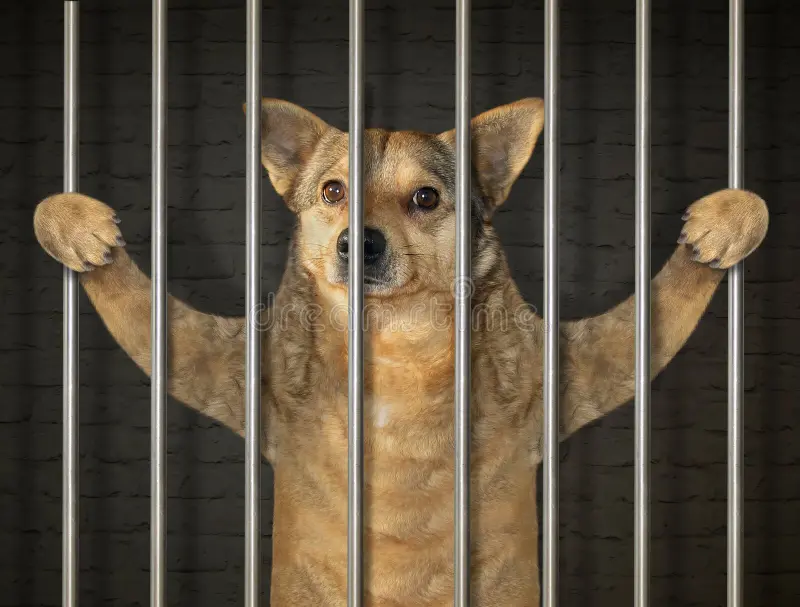
\includegraphics[width=0.8\linewidth]{plano_electrico.png}
\caption{Plano eléctrico con conexiones serie y paralelo.}
\label{fig:plano_elec}
\end{figure}

\subsection{Cálculos eléctricos}
Se asume una fuente de 120 V~CD y lámparas de 60 W cada una. La resistencia de cada lámpara se obtiene de \( R = V^2 / P = 120^2 / 60 = 240\ \Omega \).

\subsubsection{Circuito en serie}
Resistencia equivalente: \( R_{eq} = 240 + 240 + 240 = 720\ \Omega \).  
Corriente total: \( I = V / R_{eq} = 120 / 720 = 0.1667\ \text{A} \).  
Voltaje en cada lámpara: \( V_{\text{lámpara}} = I \cdot R = 0.1667 \cdot 240 = 40\ \text{V} \).  
Potencia real en cada lámpara: \( P = I^2 R = (0.1667)^2 \cdot 240 = 6.67\ \text{W} \) (brillo reducido).  
Potencia total: \( 20\ \text{W} \).

\subsubsection{Circuito en paralelo}
Resistencia equivalente: \( 1/R_{eq} = 1/240 + 1/240 + 1/240 = 3/240 \Rightarrow R_{eq} = 80\ \Omega \).  
Corriente total: \( I = 120 / 80 = 1.5\ \text{A} \).  
Corriente por lámpara: \( I_{\text{lámpara}} = 120 / 240 = 0.5\ \text{A} \).  
Potencia por lámpara: \( P = 120 \cdot 0.5 = 60\ \text{W} \) (nominal).  
Potencia total: \( 180\ \text{W} \).  
Consumo estimado en 5 horas diarias: \( 180\ \text{W} \times 5\ \text{h} = 0.9\ \text{kWh/día} \).

La Tabla \ref{tab:calculos} resume los resultados.

\begin{table}[h]
\centering
\caption{Comparativa de cálculos eléctricos.}
\label{tab:calculos}
\begin{tabular}{|l|c|c|}
\hline
\textbf{Parámetro} & \textbf{Serie} & \textbf{Paralelo} \\
\hline
\( R_{eq} \) & 720 Ω & 80 Ω \\
\( I_{\text{total}} \) & 0.1667 A & 1.5 A \\
\( V_{\text{lámpara}} \) & 40 V & 120 V \\
\( P_{\text{lámpara}} \) & 6.67 W & 60 W \\
\( P_{\text{total}} \) & 20 W & 180 W \\
\hline
\end{tabular}
\end{table}

\section{Simulación y análisis de resultados}
Los circuitos se simularon en [software]. La Figura \ref{fig:sim_serie} muestra el circuito serie con sus mediciones; la Figura \ref{fig:sim_paralelo} el circuito paralelo.

\begin{figure}[h]
\centering
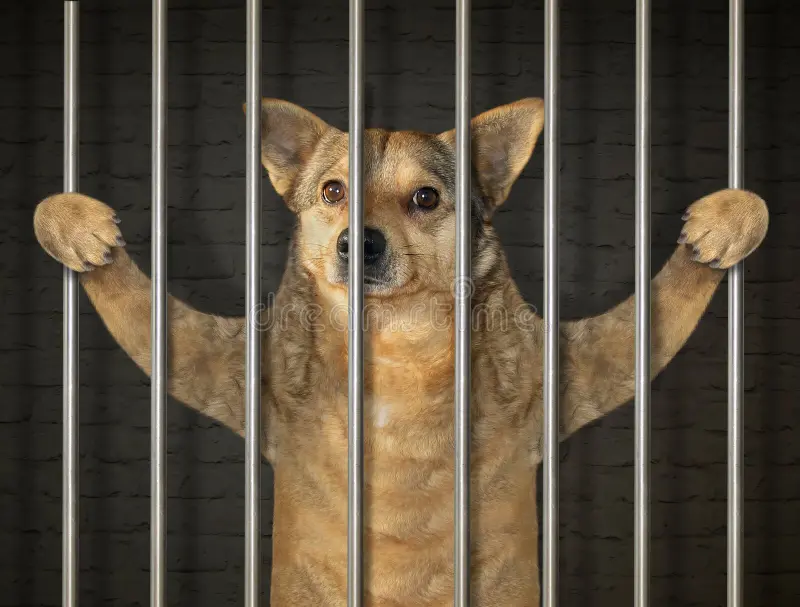
\includegraphics[width=0.7\linewidth]{simulacion_serie.png}
\caption{Simulación del circuito serie (voltajes y corriente).}
\label{fig:sim_serie}
\end{figure}

\begin{figure}[h]
\centering
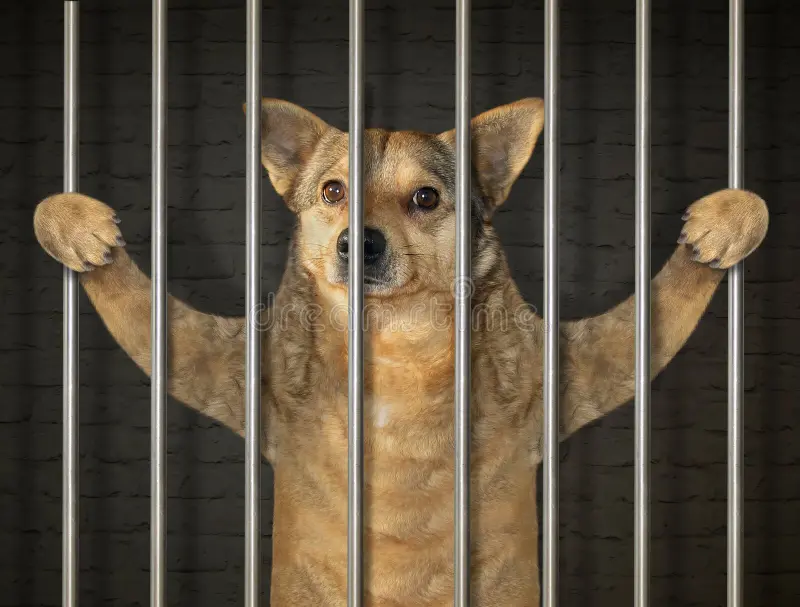
\includegraphics[width=0.7\linewidth]{simulacion_paralelo.png}
\caption{Simulación del circuito paralelo.}
\label{fig:sim_paralelo}
\end{figure}

\subsection{Comportamiento del circuito serie}
\begin{itemize}
    \item La corriente es uniforme y reducida (0.1667 A).
    \item El voltaje se divide equitativamente (40 V por lámpara), por lo que el brillo es muy bajo (≈11\% de la potencia nominal).
    \item Si una lámpara se funde, el circuito se abre y todas se apagan (dependencia total).
    \item No es adecuado para iluminación general.
\end{itemize}

\subsection{Comportamiento del circuito paralelo}
\begin{itemize}
    \item Cada lámpara recibe 120 V y opera a su potencia nominal (60 W).
    \item La corriente total es mayor (1.5 A), pero cada rama es independiente.
    \item La falla de una lámpara no afecta a las demás.
    \\item Topología estándar en instalaciones reales.
\end{itemize}

\subsection{Comparativa}
La Tabla \ref{tab:comparativa} resume ventajas y desventajas.

\begin{table}[h]
\centering
\caption{Ventajas y desventajas de cada conexión.}
\label{tab:comparativa}
\begin{tabular}{|l|c|c|}
\hline
\textbf{Aspecto} & \textbf{Serie} & \textbf{Paralelo} \\
\hline
Brillo & Muy bajo & Nominal \\
Independencia de fallas & No & Sí \\
Corriente total & Baja & Mayor \\
Caída de tensión & Alta & Nula \\
Aplicación típica & Decorativo / Navideño & Instalaciones residenciales/comerciales \\
\hline
\end{tabular}
\end{table}

\section{Lista de materiales y equipos}
\begin{itemize}
    \item Lámparas incandescentes de 60 W / 120 V (3 uds.)
    \item Interruptores unipolares (2 uds., uno para cada circuito)
    \item Cable calibre \#14 AWG (cantidad según diseño)
    \item Fuente de alimentación de 120 V~CD (o toma domiciliaria con transformador)
    \item Software de simulación: [nombre]
    \item Herramientas de dibujo: AutoCAD, QCAD o similar
    \item Cámara fotográfica
    \item Cinta métrica
\end{itemize}

\section{Evidencias}
Las evidencias fotográficas del trabajo de campo se presentan en las Figuras \ref{fig:foto1} a \ref{fig:foto3}. Incluyen el espacio real, las luminarias existentes, interruptores y el cableado visible. Los planos originales y las capturas de simulación se adjuntan en los anexos.

\begin{figure}[h]
\centering
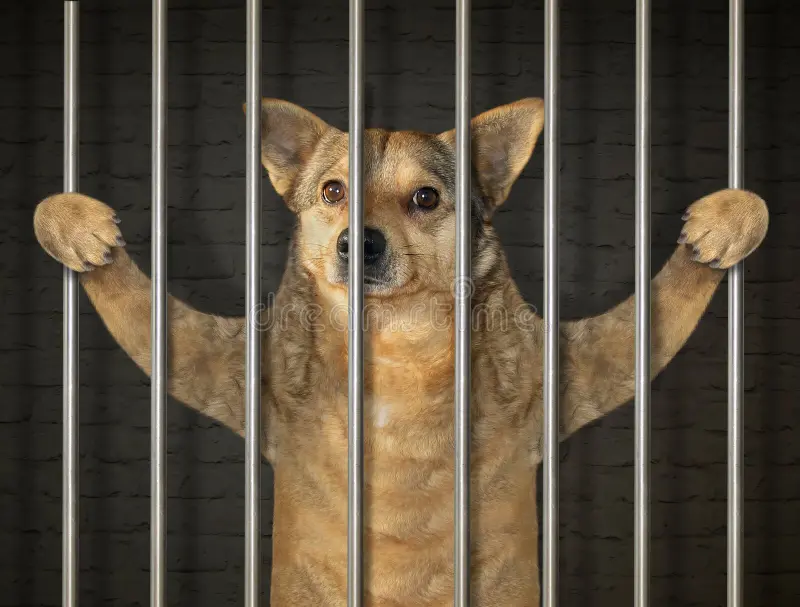
\includegraphics[width=0.6\linewidth]{foto_lugar.jpg}
\caption{Vista general del espacio.}
\label{fig:foto1}
\end{figure}

\begin{figure}[h]
\centering
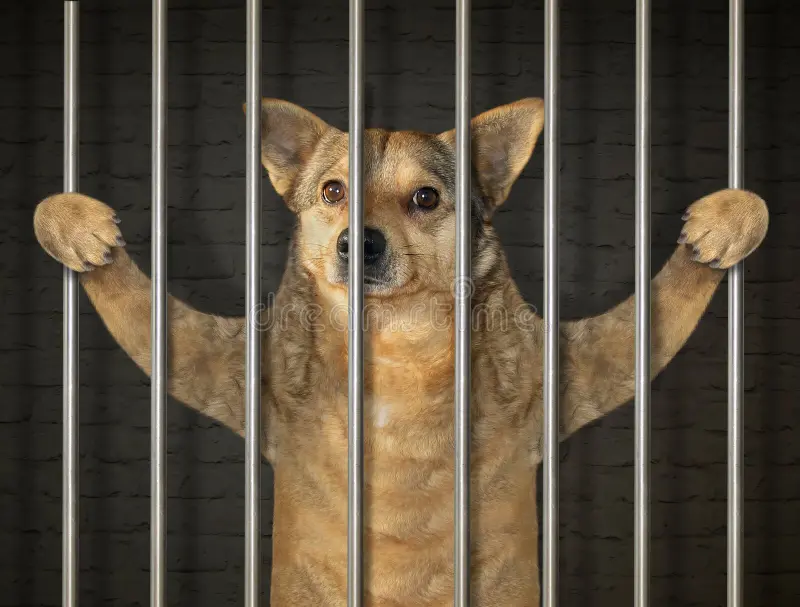
\includegraphics[width=0.6\linewidth]{foto_luminaria.jpg}
\caption{Tipo de lámpara existente.}
\label{fig:foto2}
\end{figure}

\begin{figure}[h]
\centering
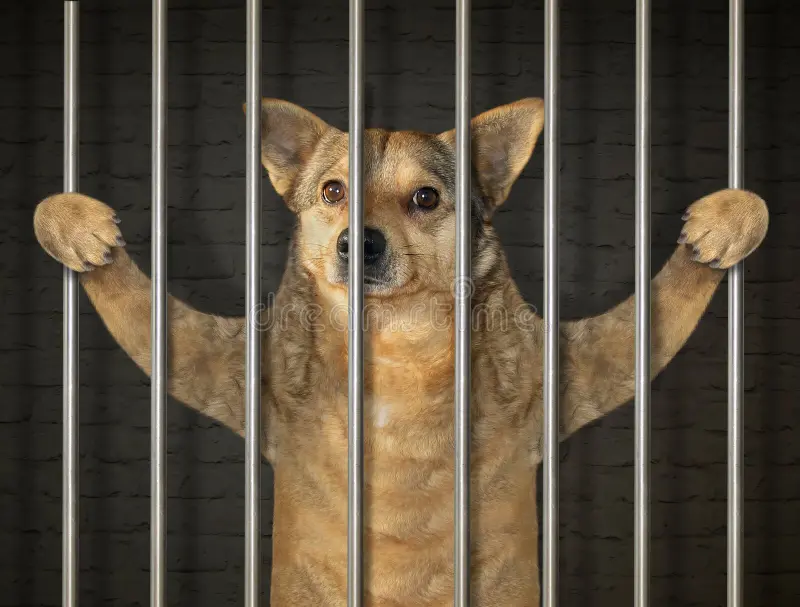
\includegraphics[width=0.6\linewidth]{foto_interruptor.jpg}
\caption{Ubicación de interruptores y cableado.}
\label{fig:foto3}
\end{figure}

\section{Conclusiones}
\begin{itemize}
    \item El levantamiento de campo permitió obtener dimensiones reales y el estado actual de la iluminación, identificando oportunidades de mejora (poca eficiencia, cableado expuesto).
    \item Los cálculos demostraron que la conexión en serie subalimenta las lámparas (40 V en lugar de 120 V) e introduce dependencia total; no es viable para iluminación funcional.
    \item La conexión en paralelo garantiza voltaje nominal en cada lámpara, operación independiente y mayor fiabilidad, siendo la topología adecuada para la instalación propuesta.
    \item La simulación validó los cálculos teóricos y facilitó la comparación visual del comportamiento eléctrico.
    \item Se recomienda implementar el diseño paralelo con interruptores independientes para cada zona, y mejorar el cableado existente según normativa.
\end{itemize}


\section*{Anexos}
Anexo A: Plano arquitectónico original (escala 1:50).  
Anexo B: Plano eléctrico con detalles de conexionado.  
Anexo C: Archivos de simulación (carpeta complementaria).



%% ─── Referencias ────────────────────────────────────────────────────────────
\nocite{*}
\bibliographystyle{apalike}
\bibliography{referencias}

\end{document}


